\chapter{Medición de tiempos de ejecución}

\section{Introducción}
Se ha mencionado en el capítulo anterior que el programa de extracción de puntos SIFT, $sift\_keypoints$, consta de dos partes principales entre otras como pueden ser cargar librerías, crear o modificar ficheros de texto. Estas dos partes son la extracción de vectores normales a la superficie descrita por la nube de puntos con la que trabaja el programa y la estimación de puntos SIFT.


En este capítulo se va a presentar una forma sencilla de medir los tiempos de ejecución de estos dos procesos a la vez que se modifican los parámetros que influyen en ellos. De este modo, se determinará si será la estimación de normales o la de puntos SIFT la parte que necesita ser llevada a hardware digital para su posterior optimización. Estas pruebas se van a realizar sobre la FPGA puesto que es en este hardware donde se desarrollarán los objetivos principales del TFG.

Además, se ha creado la sección \ref{resultados_graficos} dada la gran cantidad de ellos que hay.


\section{Método de medición}
Trabajando en C++, como de costumbre, el proceso de medición de tiempos requiere la inclusión de la librería $ctime$ para lo cual se tiene al comienzo del código en $sift\_keypoints.cpp$.

\begin{lstlisting}[language=C++,breaklines]
	#include <ctime>
\end{lstlisting}

Incluída esta librería, ahora se pueden utilizar las variables globales $begin$,$end$ y $elapsed\_sec$ declaradas de la siguiente manera:

\begin{lstlisting}[language=C++,breaklines]
	clock_t begin,end;
	double elapsed_sec;
\end{lstlisting}

Las variables $begin$ y $end$ son del tipo $clock\_t$ y sirven para almacenar cuentas de $clock\;\; ticks$ o ciclos de reloj mientras que $elapsed\_sec$ es del tipo double para almacenar el tiempo en segundos que ha llevado efectuar una determinada operación.\\
El proceso de medición de tiempo es el siguiente: 

\begin{lstlisting}[language=C++,breaklines]
	begin = clock();
	process();
	end = clock();
	
	elapsed_sec = double(end - begin)/CLOCKS_PER_SEC;
\end{lstlisting}

En primer lugar se almacena en $begin$ el valor devuelto por la función $clock()$, es decir, número de ciclos de reloj que han transcurrido en el procesador desde el inicio del programa hasta su llamada. A continuación se ejecuta el proceso cuyo tiempo de ejecución desea medirse, para este ejemplo, $process()$. Ahora se actúa de manera similar al primer paso ya que se almacena en $end$ el número de ciclos transcurridos desde el inicio del programa hasta la llamada a $clock()$ después de haberse ejecutado $process()$. Por último, se toma la diferencia de ciclos entre $end$ y $begin$ para saber cuántos ciclos ha tomado la ejecución de $process()$. Sin embargo esto no es una medida directa de tiempo por lo que el número de ciclos de ejecución del proceso se divide entre una constante, el número de ciclos que duran un segundo y que se llama $CLOCKS\_PER\_SEC$. El resultado se almacena en $elapsed\_sec$ como el tiempo en segundos que ha durado la ejecución de $process()$.


\section{Resultados de medición sobre la FPGA}
Una vez visto cómo se mide el tiempo de ejecución de cualquier parte del programa $sift\_keypoints$, se rescata parte del código del mismo para indicar qué procesos van a ser sometidos a esta medición.


En la parte de estimación de normales se analiza el método $compute$ el cual realiza todas las operaciones pertinentes para almacenar en $cloud\_normals$ los vectores normales a partir de $cloud\_xyz$:


\begin{lstlisting}[language=C++,breaklines]
  pcl::PointCloud<pcl::PointNormal>::Ptr cloud_normals (new 		pcl::PointCloud<pcl::PointNormal>);
  pcl::search::KdTree<pcl::PointXYZ>::Ptr tree_n(new pcl::search::KdTree<pcl::PointXYZ>());

  ne.setInputCloud(cloud_xyz);
  ne.setSearchMethod(tree_n);
  ne.setRadiusSearch(radius_search);
 
  std::cout << "Estimating normals in " << filename << " surface..." <<std::endl;

  begin = clock();
  ne.compute(*cloud_normals);
  end = clock();

  normal_estimation_time = double(end-begin)/CLOCKS_PER_SEC;
  std::cout << "Time needed for normal estimation (compute) in " << filename << ": " << normal_estimation_time << " seconds" << std::endl << std::endl;
\end{lstlisting}

Se procede de forma análoga en la parte de estimación de puntos SIFT puesto que, tras establecer el valor de los parámetros también se llama a un método $compute$ para efectuar la extracción de keypoints:

\begin{lstlisting}[language=C++,breaklines]
  pcl::SIFTKeypoint<pcl::PointNormal, pcl::PointWithScale> sift;
  pcl::PointCloud<pcl::PointWithScale>::Ptr result(new pcl::PointCloud<pcl::PointWithScale>);
  pcl::search::KdTree<pcl::PointNormal>::Ptr tree(new pcl::search::KdTree<pcl::PointNormal> ());
  sift.setSearchMethod(tree);
  sift.setScales(min_scale, n_octaves, n_scales_per_octave);
  sift.setMinimumContrast(min_contrast);
  sift.setInputCloud(cloud_normals);
 
  std::cout << "Estimating sift points in " << filename << "..." << std::endl;

  begin = clock();
  sift.compute(*result);
  end = clock();
  sift_estimation_time = double(end-begin)/CLOCKS_PER_SEC;
  std::cout << "Time needed for sift point extraction: " << sift_estimation_time << " seconds" << std::endl << std::endl;
\end{lstlisting}

Los tiempos de ejecución del método $compute$ se almacenan en $normal\_estimation\_time$ y $sift\_estimation\_time$ para la parte de estimación de normales y puntos SIFT, respectivamente.
\\
Para aportar mayor amplitud a los resultados obtenidos, se van a realizar mediciones de los métodos $compute$ variando ligeramente los parámetros involucrados en la estimación de normales y puntos SIFT. Como se ha visto en los fragmentos de código mostrados, la extracción de normales varía con un único parámetro, $radius\_search$, mientras que el tiempo de estimación de keypoints varía con $min\_scale$, $n\_octaves$ y $n\_scales\_per\_octave$. El parámetro $min\_contrast$ no afecta al tiempo del proceso estudiado porque, como se ha visto anteriormente, indica la dureza de la criba de los puntos SIFT ya obtenidos.

Las nubes sobre las que se han realizado las pruebas son las mismas que las mostradas en el capítulo anterior: $bunny.pc$, $cturtle.pcd$ y $milk\_cartoon\_all\_small\_clorox.pcd$

Tras efectuar la medición de tiempos junto a la variación de parámetros, éstos se han plasmado en diferentes gráficas. En primer lugar, se analizan los tiempos de estimación de normales y puntos SIFT variando el parámetro $radius\_search$ puesto que la extracción de normales es la primera operación y afecta a las que vienen después. El resultado se aprecia en las figuras \ref{fig:grafico_radius_bunny}, \ref{fig:grafico_radius_cturtle} y \ref{fig:grafico_radius_milk} las cuales indican que en todos los casos un incremento del radio de búsqueda de normales a la superficie dispara el tiempo de computación mientras que el tiempo de extracción de puntos SIFT se mantiene entorno a un valor estable a pesar de que la cantidad de normales extraídas afecta a la estimación de keypoints. Resulta obvio este incremento del tiempo de computación ya que la información que hay que utilizar para estimar un vector normal se incrementa, es decir, se considera una porción de la superficie de la nube cada vez más grande.



Se muestra en las figuras \ref{fig:grafico_min_scale_bunny}, \ref{fig:grafico_min_scale_cturtle} y \ref{fig:grafico_min_scale_milk} cómo varían estos mismos tiempos modificando el parámetro $min\_scale$. Se tiene en esta ocasión algo más de variedad en los resultados obtenidos ya que en $cturtle.pcd$ y $bunny.pcd$ el tiempo de estimación de keypoints comienza siendo mayor que el de extracción de normales pero a medida que incrementa $min\_scale$ éste decrece considerablemente. Esto se debe a que la nube de entrada se convoluciona con un filtro Gaussiano cada vez más severo, es decir, un aumento de la desviación típica difumina en mayor medida la nube y hace que ésta pierda detalles finos por lo que los puntos SIFT se encuentran en esquinas o bordes muy marcados y nítidos que son capaces de persistir ante el filtro aplicado. Por otra parte, el tiempo de estimación de normales no varía ya que su único parámetro, $radius\_search$, a partir de ahora tomará el valor por defecto. En cuanto a nubes a nubes con mayor nivel de detalle y cantidad de información como en $milk\_cartoon\_all\_small\_clorox.pcd$, se puede ver que aumentar el parámetro $min\_scale$ disminuye el tiempo de estimación de puntos SIFT siendo éste ya notablemente menor que el de extracción de normales.




Ahora se modifica el parámetro $n\_octaves$ y se aprecia que para casos realistas (nubes que contienen una gran cantidad de puntos como las nubes $milk\_cartoon\_all\_small\_clorox.pcd$ y $cturtle.pcd$) como se indican en las figuras \ref{fig:grafico_n_octaves_cturtle} y \ref{fig:grafico_n_octaves_milk} el tiempo de estimación de normales es en todo caso superior al de extracción de puntos SIFT incluso aunque se afine esta búsqueda aportando  más octavas en las que estimar keypoints. No es así en una nube pequeña como $bunny.pcd$ lo cual se puede considerar un caso particular tal y como indica la figura \ref{fig:grafico_n_octaves_bunny}.



Por último, se estudia el tiempo de estimación de keypoints ante la variación del parámetro $n\_scales\_per\_octave$ apreciándose los resultados en las figuras \ref{fig:grafico_n_scales_bunny}, \ref{fig:grafico_n_scales_cturtle} y \ref{fig:grafico_n_scales_milk}. Se tiene de nuevo un tiempo de estimación de normales predominante ante la extracción de puntos SIFT para nubes con una cantidad considerable de puntos como $cturtle.pcd$ y $milk\_cartoon\_all\_small\_clorox.pcd$. En esta ocasión, incrementar el número de convoluciones de la nube por octava implica realizar más operaciones y tener en cuenta la misma nube bajo más filtros para extraer keypoints por lo que el tiempo implicado en este proceso aumenta.


\section{Conclusiones}
Habiendo estudiado cómo varían los tiempos de estimación de normales y puntos SIFT con diferentes valores de los parámetros implicados se concluye que se va a desarrollar hardware digital para su posterior optimización sobre la parte de extracción de vectores normales a la superficie representada por la nube de puntos. Esto es así por dos motivos:

\begin{itemize}
\item[•]Para nubes de puntos de gran tamaño, el tiempo de estimación de normales predomina sobre el de extracción de puntos SIFT.
\item[•]La estimación de vectores normales solamente varía bajo la acción de un parámetro, $radius\_search$, mientras que la extracción de puntos SIFT es más flexible puesto que está sometida a tres parámetros: $min\_scale$, $n\_octaves$ y $n\_scales\_per\_octave$.
\end{itemize}

En el siguiente capítulo se estudiará a fondo el algoritmo de extracción de normales puesto que se ha elegido éste para ser optimizado tras su síntesis en hardware digital.

\section{Resultados gráficos}\label{resultados_graficos}

\begin{figure}[h!]
\centering
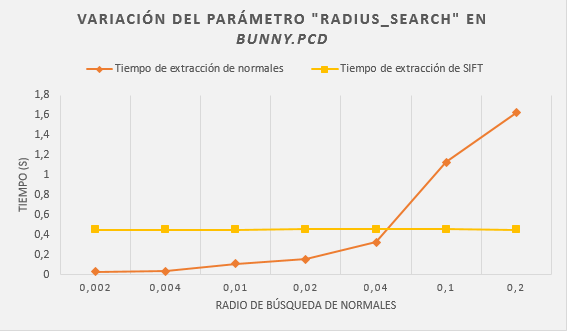
\includegraphics[scale=1]{grafico_radius_bunny}
\caption{Tiempos de estimación de normales y puntos SIFT en $bunny.pcd$ variando $radius\_search$.}\label{fig:grafico_radius_bunny}
\end{figure}

\begin{figure}[h!]
\centering
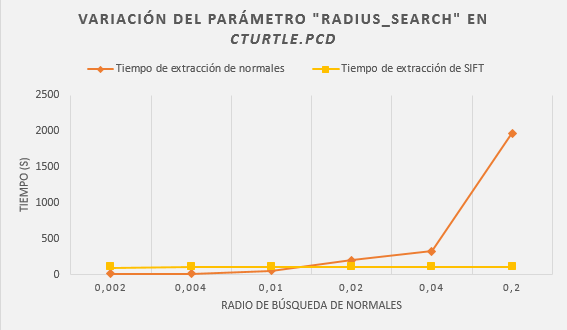
\includegraphics[scale=1]{grafico_radius_cturtle}
\caption{Tiempos de estimación de normales y puntos SIFT en $cturtle.pcd$ variando $radius\_search$.}\label{fig:grafico_radius_cturtle}
\end{figure}


\begin{figure}[h!]
\centering
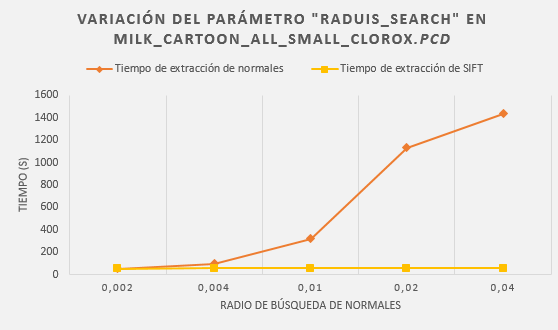
\includegraphics[scale=1]{grafico_radius_milk}
\caption{Tiempos de estimación de normales y puntos SIFT en $milk\_cartoon\_all\_small\_clorox.pcd$ variando $radius\_search$.}\label{fig:grafico_radius_milk}
\end{figure}


\begin{figure}[h!]
\centering
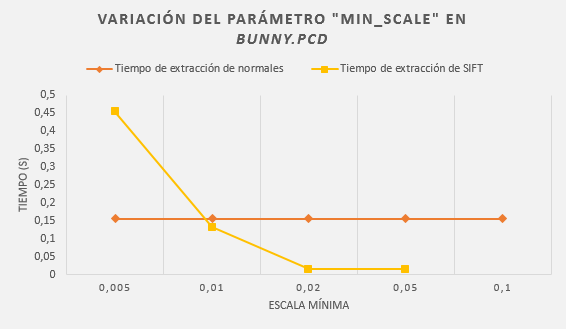
\includegraphics[scale=1]{grafico_min_scale_bunny}
\caption{Tiempos de estimación de normales y puntos SIFT en $bunny.pcd$ variando $min\_scale$.}\label{fig:grafico_min_scale_bunny}
\end{figure}

\begin{figure}[h!]
\centering
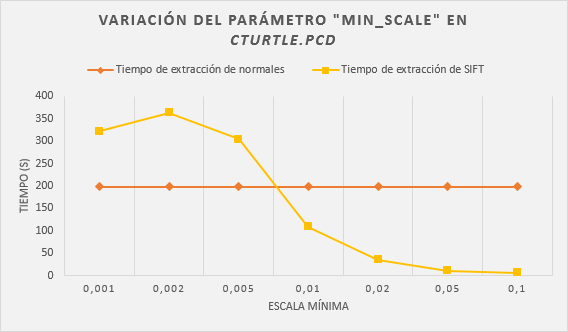
\includegraphics[scale=1]{grafico_min_scale_cturtle}
\caption{Tiempos de estimación de normales y puntos SIFT en $cturtle.pcd$ variando $min\_scale$.}\label{fig:grafico_min_scale_cturtle}
\end{figure}


\begin{figure}[h!]
\centering
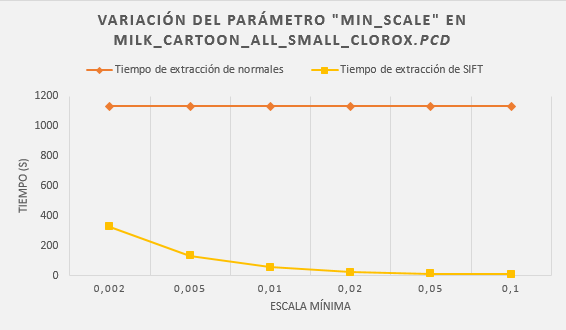
\includegraphics[scale=1]{grafico_min_scale_milk}
\caption{Tiempos de estimación de normales y puntos SIFT en $milk\_cartoon\_all\_small\_clorox.pcd$ variando $min\_scale$.}\label{fig:grafico_min_scale_milk}
\end{figure}


\begin{figure}[h!]
\centering
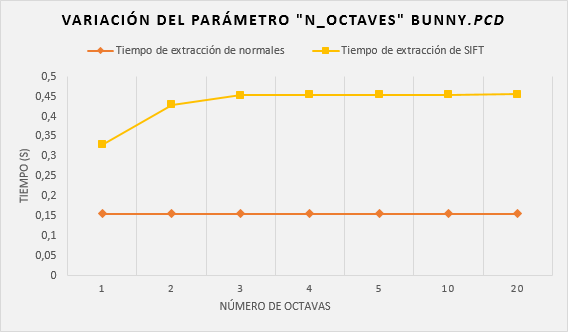
\includegraphics[scale=1]{grafico_n_octaves_bunny}
\caption{Tiempos de estimación de normales y puntos SIFT en $bunny.pcd$ variando $n\_octaves$.}\label{fig:grafico_n_octaves_bunny}
\end{figure}

\begin{figure}[h!]
\centering
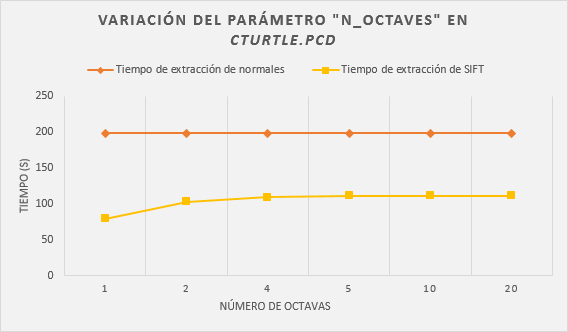
\includegraphics[scale=1]{grafico_n_octaves_cturtle}
\caption{Tiempos de estimación de normales y puntos SIFT en $cturtle.pcd$ variando $n\_octaves$.}\label{fig:grafico_n_octaves_cturtle}
\end{figure}

\begin{figure}[h!]
\centering
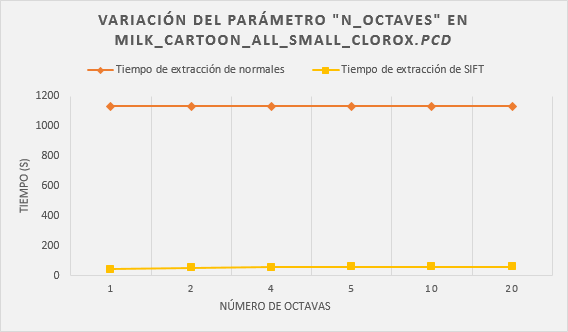
\includegraphics[scale=1]{grafico_n_octaves_milk}
\caption{Tiempos de estimación de normales y puntos SIFT en $milk\_cartoon\_all\_small\_clorox.pcd$ variando $n\_octaves$.}\label{fig:grafico_n_octaves_milk}
\end{figure}


\begin{figure}[h!]
\centering
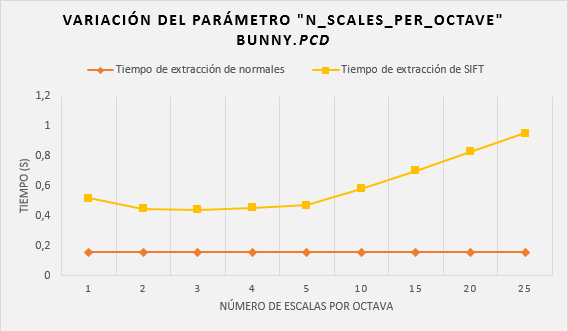
\includegraphics[scale=1]{grafico_n_scales_bunny}
\caption{Tiempos de estimación de normales y puntos SIFT en $bunny.pcd$ variando $n\_scales\_per\_octave$.}\label{fig:grafico_n_scales_bunny}
\end{figure}

\begin{figure}[h!]
\centering
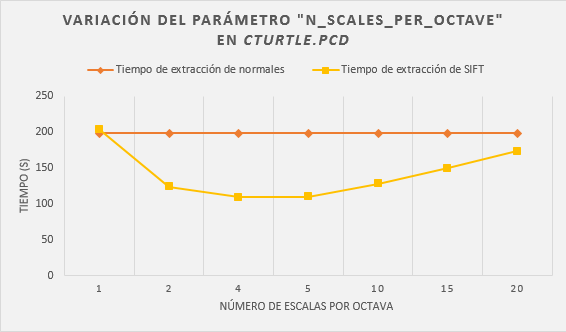
\includegraphics[scale=1]{grafico_n_scales_cturtle}
\caption{Tiempos de estimación de normales y puntos SIFT en $cturtle.pcd$ variando $n\_scales\_per\_octave$.}\label{fig:grafico_n_scales_cturtle}
\end{figure}


\begin{figure}[h!]
\centering
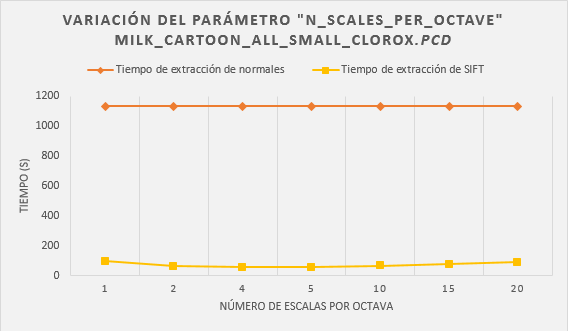
\includegraphics[scale=1]{grafico_n_scales_milk}
\caption{Tiempos de estimación de normales y puntos SIFT en $milk\_cartoon\_all\_small\_clorox.pcd$ variando $n\_scales\_per\_octave$.}\label{fig:grafico_n_scales_milk}
\end{figure}


